\documentclass{beamer}
%\documentclass[presentation]{beamer}
\setbeamercovered{transparent}
\usecolortheme{Imperial}
 
\usepackage[utf8]{inputenc}
\usepackage[UKenglish]{babel}
\usepackage{booktabs}
\usepackage{caption}
\usepackage{subcaption}
\usepackage{graphicx}
\usepackage{amsmath}
\usepackage{amsfonts}
\usepackage{amssymb}
\usepackage{epstopdf}

% complying UK date format, i.e. 1 January 2001
\usepackage{datetime}
\let\dateUKenglish\relax
\newdateformat{dateUKenglish}{\THEDAY~\monthname[\THEMONTH] \THEYEAR}

% Imperial College Logo, not to be changed!
\institute{
\includegraphics[height=0.7cm]{Imperial_1_Pantone_solid.eps}}

% -----------------------------------------------------------------------------




%Information to be included in the title page:
\title{Week 1}

%\subtitle{Subtitle}

\author{Elise Özalp}
%\setbeamercovered{transparent}
\date{\today}



\begin{document}
 
\frame{\titlepage}


\begin{frame}
	\frametitle{Lorenz System}
	\begin{align*}
	    \frac{dx}{dt} &= \sigma(y-x)\\
	    \frac{dy}{dt} &= x(\rho-z) -y \\
	    \frac{dz}{dt} &= xy -\beta z 
	\end{align*}
	\begin{itemize}
	       \item$ \sigma = 10, \beta = 8/3, \rho = 28 $
	    \item Initial condition $(0, 1, 1)$
	    \item Time: $[0, 100], \Delta t = 0.001$
	\end{itemize}

\end{frame}


\begin{frame}

\begin{figure}
    \centering
    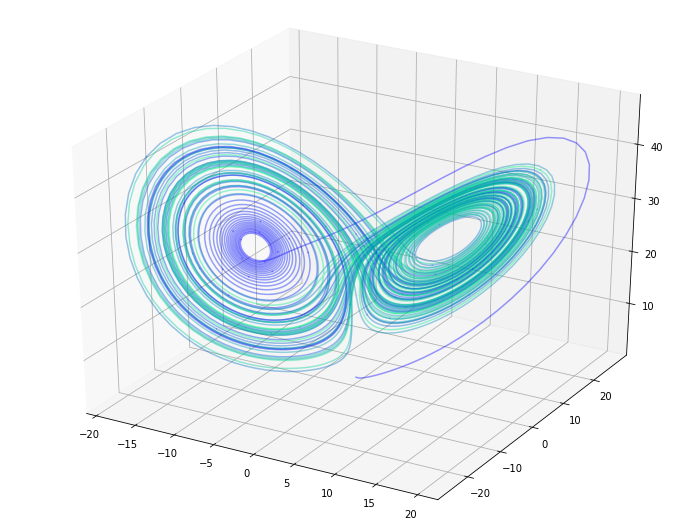
\includegraphics[width=0.8\textwidth]{Lorenz_system_init1.png}
    \caption{Solution of Lorenz System, Method: explicit RK of order 5}
    \label{fig:my_label}
\end{figure}

\end{frame}


\begin{frame}
	\begin{figure}
	    \centering
	    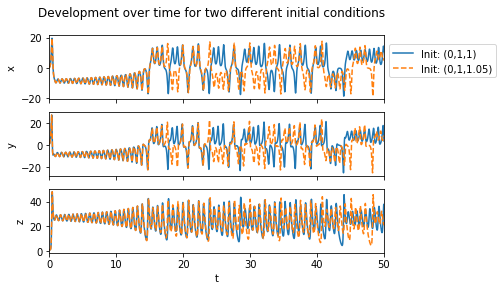
\includegraphics[width=0.9\textwidth]{two_init_lorenz.png}
	    \caption{Comparison with second initial condition}
	    %\label{fig:my_label}
	\end{figure}
\end{frame}

\begin{frame}{Implementation}
\begin{itemize}
    \item Implementation in Python
    \item Solver using Scipy (RK, order 5)
    \item Save time, solution using Numpy
\end{itemize}
\end{frame}


\begin{frame}{Questions}
\begin{itemize}
    \item What is the goal of the PI-LSTM prediction? 
     \item Reference: \textit{Short- and long-term predictions of chaotic flows and extreme events: a physics-constrained reservoir computing approach}

    
\end{itemize}
    
\end{frame}
\begin{frame}
	\frametitle{Connection to physics-constrained ESN}
Dynamical system:
\begin{align}
    &\dot{y} = \mathcal{N}(y) \\
    & y(0) = y_0
\end{align}
\pause
Training data:
\begin{itemize}

    \item input time series $u(n) \in \mathbb{R}^{N_u}$
    \item target time series $y(n) \in \mathbb{R}^{N_y}$
\end{itemize}
with discrete time instants $n=0, \dots N_t$ from $0$ to $T=N_t\Delta t$.
\end{frame}



 \begin{frame}{Questions}
 Training data:
\begin{itemize}
    \item input time series $u(n) \in \mathbb{R}^{N_u}$
    \item target time series $y(n) \in \mathbb{R}^{N_y}$
\end{itemize}
with discrete time instants $n=0, \dots N_t$ from $0$ to $T=N_t\Delta t$.
\newline
\begin{itemize}
    \item Can you explain the training data?
    \pause
    \item Why time-series approach instead of using information about $t$?
    \pause
    \item How do we prepare Lorenz data for LSTM?
    
\end{itemize}
    
\end{frame}
 \begin{frame}%{Replace ESN by LSTM?}
 \begin{figure}
     \centering
     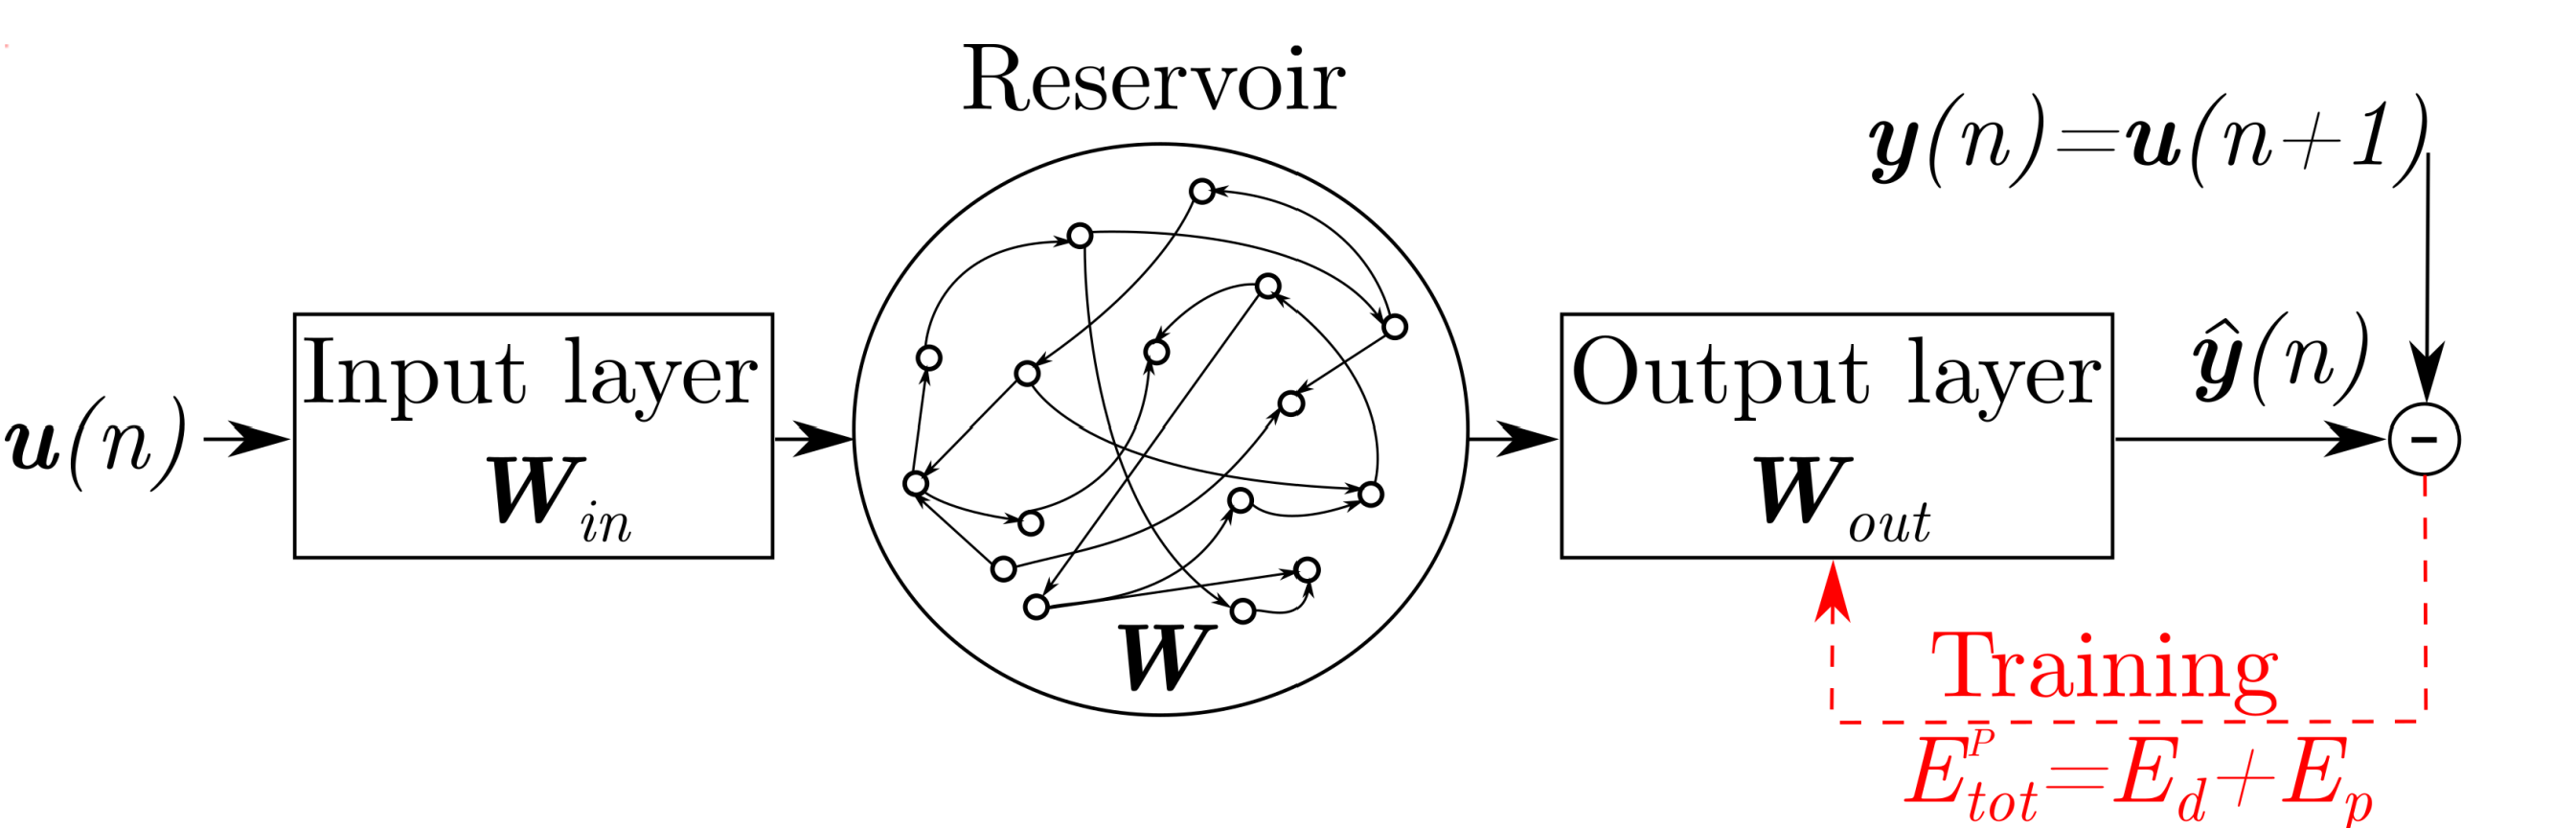
\includegraphics[width=\textwidth]{ESN_training.png}
     \caption{Training of physics-constrained ESN}
     %\label{fig:my_label}
 \end{figure}

    
\end{frame}

 \begin{frame}{Replace ESN by LSTM?}
 \begin{figure}
     \centering
     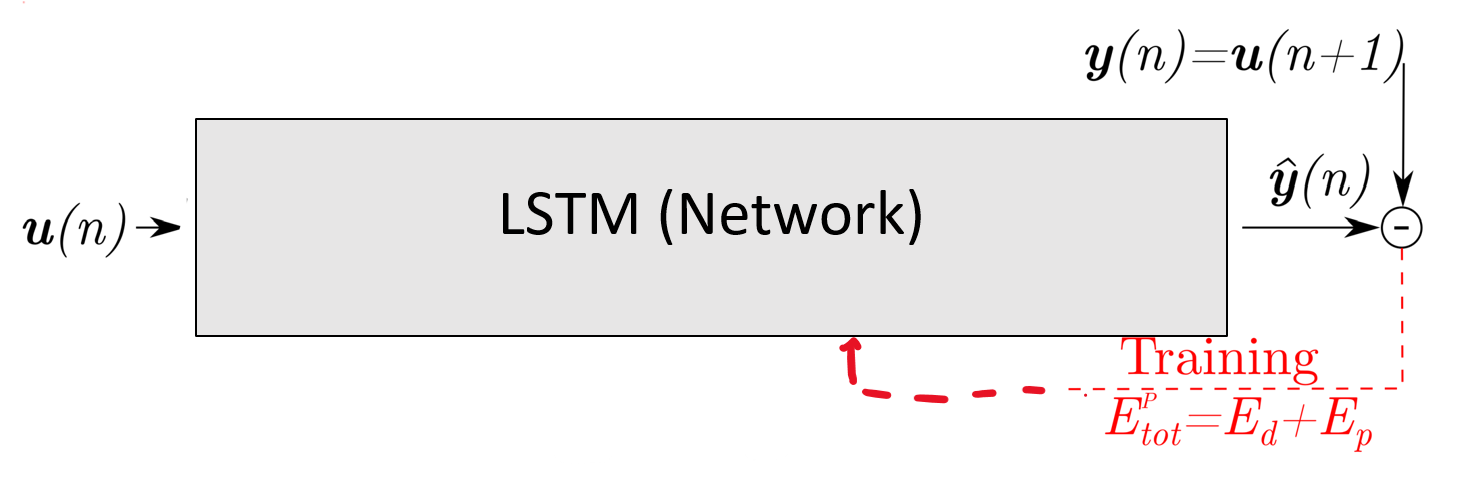
\includegraphics[width=\textwidth]{LSTM_training.png}
     \caption{Training of physics-constrained LSTM}
     %\label{fig:my_label}
 \end{figure}

    
\end{frame}


\end{document}

